\documentclass[10pt]{sensys-proc}

\usepackage{graphicx}
\usepackage{color}
\usepackage{cite}
\usepackage{balance}
\usepackage{amsmath}
\usepackage{algorithm}
\usepackage{algpseudocode}
\usepackage{multirow}
\usepackage{url}
\floatname{algorithm}{Procedure}

%%%%%% FOR DRAFT VERSION - REMOVE FOR FINAL VERSION %%%%%%%%%%%%%%%%%%%%%%
\usepackage{lastpage} % for the number of the last page in the document  %
\usepackage{fancyhdr}                                                    %
\pagestyle{fancy}                                                        %
\fancyhf{}                                                               %
\lhead{--- DRAFT ---}                                                    %
\rhead{Section \thesection}                                              %
\lfoot{\today}                                                           %
\rfoot{Page \thepage\ of \pageref{LastPage}}                             %
%%%%%%%%%%%%%%%%%%%%%%%%%%%%%%%%%%%%%%%%%%%%%%%%%%%%%%%%%%%%%%%%%%%%%%%%%%

\newcommand{\redtext}[1]{\textcolor{red}{#1}}
\newcommand{\rednote}[1]{\textcolor{red}{\small #1}}
\newcommand{\degc}{\ensuremath{\,^{\circ}\mathrm{C}}}
%\newcommand{\aPoint}[1]{\vspace{.5\baselineskip} \noindent\textbf{[#1]}} %Chung-Yi

\numberofauthors{2}

%\author{ %anon style
%{Scribus Primus}\\
%\affaddr{Primus Address}\\
%\emai	l{primus@somewhere.com} \and
%{Scribus Secundus}\\
%\affaddr{Secundus Address}\\
%\email{secondus@elsewhere.com}
%}
%

%\author{ % ntu/intel separated style
%{Chung-Yi Li, Wei-Lun Su, Todd G.\ McKenzie, Fu-Chun Hsu, %students
%Shou-De Lin, Jane Yung-jen Hsu}\\ %professors
%\affaddr{Department of Computer Science and Information Engineering, National Taiwan University, Taiwan}\\
%\email{\{r00922051,r00922050,d97041,r94082,sdlin,yjhsu\}@csie.ntu.edu.tw} \and
%{Phillip B.\ Gibbons}\\
%\affaddr{Intel Research Pittsburgh, USA}\\
%\email{phillip.b.gibbons@intel.com}
%}

\author{ % ntu/intel combined style
{Chung-Yi Li$^1$, Wei-Lun Su$^1$, Todd G.\ McKenzie$^1$, Fu-Chun Hsu$^1$,}\and %students
{Shou-De Lin$^1$, Phillip B.\ Gibbons$^2$, Jane Yung-jen Hsu$^1$}\vspace{3pt}\\ %professors + phil
\affaddr{$^1$Department of Computer Science and Information Engineering, National Taiwan University, Taiwan}\\
\email{\{r00922051,r00922050,d97041,r94082,sdlin,yjhsu\}@csie.ntu.edu.tw}\\
\affaddr{$^2$Intel Research Pittsburgh, USA}\\
\email{phillip.b.gibbons@intel.com}
}

\title{A Collaborative Filtering Approach\\to Estimating Missing Sensor Data}

\crdata{978-1-4503-1169-4}
\conferenceinfo{SenSys'12,} {November 6--9, 2012, Toronto, ON, Canada.}
\CopyrightYear{2012}

\begin{document}

\maketitle
\begin{abstract}
Data sets gathered from sensor networks often suffer from a significant fraction of missing data, due to issues such as 
communication interference, sensor interference, power depletion, and hardware failure. 
Many standard data analysis tools such as classification engines, time-sequence pattern analysis modules, and even statistical 
tools are ill-equipped to deal with missing values---hence, there is a vital need for highly-accurate techniques for imputing
missing readings prior to analysis.

In this paper, we present novel imputation methods that take a ``Recommendation Systems'' view of the problem: 
the sensors and their readings at each time step are viewed as products and user product ratings, with the goal of estimating the missing ratings.
Sensor readings differ from product ratings, however, in that the former exhibit high correlation in both time and space.
To incorporate this property, we modify the widely successful Matrix Factorization (MF) approach for recommendation systems to model inter-sensor and intra-sensor correlations and learn latent relationships among these dimensions.
We evaluate the approach using two environmental sensor network datasets, one indoor and one outdoor, and
two imputation scenarios, corresponding to intermittent readings and failed sensors.
The results show that our Temporally-Regularized MF (TR-MF) approach provides significantly higher estimation accuracy than 
both (i) state-of-the-art recommendation models and (ii) state-of-the-art sensor data imputation approaches 
%such as the Applying K-nearest neighbor (AKE) model.
such as AKE.
The experiments also show that adding spatial coordinate information into TR-MF yields even better results
in the failed sensors scenario, but {\em not} in the intermittent readings scenario.

Next, we consider sensor networks with multiple sensor types at each node.  We present two techniques for extending TR-MF to account for possible correlations among sensor types (e.g., temperature and
humidity): Multivariate TR-MF and Temporally-Regularized Tensor Factorization.  Our results show that both techniques 
can significantly improve the accuracy over TR-MF, and each has its strengths, depending on the observed variance in the readings.

Finally, we consider a popular data analysis task---building regression-based prediction models---and show that,
compared to prior approaches for imputation, using TR-MF leads to a much higher quality prediction model.

\end{abstract}

%\category{H.4}{Information Systems Applications}{Miscellaneous}
%A category including the fourth, optional field follows...
%\category{D.2.8}{Software Engineering}{Metrics}[complexity measures, performance measures]

%\terms{Delphi theory}

%Omit for submission, to save space:
%\keywords{missing data recovery, matrix factorization, tensor factorization, temporal regularization, multivariate learning, data imputation}

\section{Introduction}

\subsection{Problem Statement (what is the problem to be solved?)}
We consider a centralized method of filling in missing data in sensor network datasets.
Given a complete sensor network dataset with missing data, we estimate the missing observations globally.

%\subsection{Relevance (why is WSN dataset analysis an important topic?)}
%The increasing pervasiveness of Wireless Sensor Network (WSN) deployments is reflected by the recent coinage of terms such as ``Internet of Things'' and ``Machine-to-Machine'' to describe this growing revolution~\cite{ashton2009internet,gershenfeld2004internet,nokia2004machine,lawton2004machine}.
%Facilitated by a sharp reduction in hardware costs~\cite{estrin2000special}, this growing trend (beyond providing for the admission of new phrases into the vernacular) has led to an explosion in the amount and variety of sensor network data in need of study.
%For this reason, analysis of WSN data has garnered much attention in recent years~\cite{balazinska2007data}.

\subsection{Motivation (why is data imputation needed for WSN datasets?)}
Wireless Sensor Networks are especially susceptible to interference, power failure, and other environmental and communications ailments which lead to data loss.
One important area of WSN data analysis, however, is the application of machine learning algorithms to discriminate between or predict the occurrence of events within the sensor network deployment environment.
Many of these approaches (e.g.\ \redtext{LIST ALGORITHMS HERE}) require complete datasets are unable to deal with missing values.
The filling of these missing data values (in Statistics, known as Data Imputation) is thus a vital tool in the preparation of WSN data for subsequent analysis. 
Because subsequent analyses depend on accurate sensor data to draw quality conclusions or predictions, improvement in missing sensor data estimation methodology can directly lead to better solutions to sensor network deployment objectives.

\subsection{Background (what solutions currently exist?)}
Data imputation techniques as applied to WSN datasets can be divided into four categories:
temporal methods (i.e.\ estimation using the observations from the target sensor at nearby time-steps),
spatial methods (i.e.\ estimation using neighboring sensor node observations),
heterogeneous sensor methods (i.e.\ like spatial, however now considering sensors of different types),
and hybrid methods.

\subsubsection{Temporal Methods}
The feasibility of estimating missing sensor observations based on historical data is grounded by the known temporal correlation in WSN data~\cite{akyildiz2004exploiting}.
Moreover, where there is a potential for global communication issues to affect the availability for sensor node observations \emph{en masse} during a given duration of time, utilizing spatial correlations as a basis for estimation may be not be possible.
Temporal imputation methods include observed data mean~\cite{madden2005tinydb,setz2009combining}, last seen[], linear interpolation[].
These methods suffer, however, when there are long temporal gaps of data for a given sensor (i.e.\ as can happen when intermittent communications starvation occurs in large WSNs).
As a result, the usefulness of temporal imputation methods drop rapidly as the number of consecutively missing packets becomes large.

\subsubsection{Spatial Methods}
Where spatial information is available for deployed sensor nodes, this information may be used to enforce a correlation among of neighboring sensor observations.
Methods which exploit this approach include associations rule mining~\cite{le2005estimating,jiang2007estimating} and weighting functions of nearby sensors~\cite{li2008spatial,li2008data,pan2010k}.
Generally, methods which rely solely on the spatial imputation approach suffer from the inability to estimate missing data which occurs across of many sensors simultaneously, which can occur in practice due to communication interference for example.
Spatial methods also fail to take into account barriers or other sources of sharp environmental gradients which may deter the usage of spatial information as a first-order inter-sensor node correlation approximation.
For instance, a sensor deployed in close proximity to a furnace and one deployed nearby but beneath an air-conditioning vent may be only weakly correlated by spatial information.
There is also the corollary possibility of a pair of temperature sensors deployed quite distance from one another, yet having a strong correlation due to well-circulated air flow between the two.
Certain methods consider not strictly the distance between sensors, but instead establishes a ``neighborhood of influence'' whose size becomes a tuning parameter of this approach.

\subsubsection{Heterogeneous Sensor Methods}
\redtext{more here!}

\subsubsection{Hybrid Methods}
Hybrid methods of temporal and spatial approaches are less common in the literature.
For example, the average of the temporal approach of linear interpolation and the spatial approach of multivariate regression has been reported[8].
Strictly speaking, this approach can be thought of as an ensemble approach between the two methods rather than a fully-integrated approach which considers both temporal and spatial aspects of WSN data.

%\subsection{Research Gap Identification (why are current approaches inadequate?)}
%Accurate imputation of missing sensor network observations is crucial to allow for effective subsequent analysis.
%While there are many existing algorithms which estimate missing data (as documented in the following Related Works section), few of these take advantage of the time and space dependencies inherent in the WSN datasets during the data imputation process.
%As a result, the accuracy of such approaches is limited.

\subsection{Method Overview (what is our approach to bridge the research gap?)}
In our work, we employ a novel collaborative-filtering (CF) approach to WSN data imputation inspired by the field of Recommendation Systems.
In typical CF approaches, the elements of interest are users and items, whereas WSNs are sensor node and time-steps.
Applying standard CF techniques, a sensor reading at a given time-step may be estimated much like a user rating for a given item.
Clearly a sensor reading at a given time will be correlated with itself and its neighbors at times close to that given.
It is this insight and the potential integration with CF methods which has driven the current work.
In particular, we focus on Matrix and Tensor Factorization, providing a novel method to augment these well-established techniques to exploit the temporal and spatial relationships among WSN nodes.

\subsection{Results Overview (how does our method compare to the state of the art?)}
We explore two different environmental datasets, one indoor and one outdoor.
Both datasets record temperature, humidity, and light within its deployed environment.
Each dataset has an initial missing rate (which strengthens the claim that missing data in WSNs is a common issue), to which we additionally cover known observations to use for validation and testing purposes.
Given these experimental conditions, we show that our temporal and spatial-oriented collaborative filtering approach to data imputation for WSNs performs more accurately than existing methods such as linear regression and hybrid-kNN.

\subsection{Contributions (what are the novel aspects of our work?)}
Our contributions to the body of research related to missing sensor network data estimation include:
\begin{itemize}
\item Application of the Collaborative Filtering of Recommendation Systems to the Sensor Network domain
\item Augment Collaborative Filtering with temporal coherence and multi-sensor signals (our method builds a global model incorporating intra-sensor and inter-sensor information together and directly optimizes the objective function as opposed to the piecewise combination of disparate approaches as is common in the literature.
\item Empirical study which finds that our method works well without the incorporation spatial information and that our approach can facilitate the generation of better prediction models
\item A strong argument that directly exploiting spatial information to specify the assumed inter-sensor node correlation may not be as good as directly learning these correlations directly from the sensor observations themselves.
\end{itemize}

\subsection{Paper Organization (how is the paper organized?)}
The remainder of our paper is organized as follows.
Related Work is reviewed in Section \ref{sec:rw}.
In Sections \ref{sec:mf} and \ref{sec:tf} we describe our Matrix and Tensor Factorization approaches to WSN data imputation, respectively.
Sections \ref{sec:disc} and \ref{sec:conc} provide discussion of our findings and the conclusion.

\section{Related Work} \label{sec:rw}

Related Work here!


\section{Using Matrix Factorization for Imputation}  \label{sec:mf}

% need update and to be consistent with related work, need to add the Netflix and our KDD2011 papers to support MF

Matrix Factorization (MF) is arguably the most successful Collaborative Filtering~(CF) technique in the area of Recommendation Systems~\cite{koren2009matrix, chen2011linear}. Comparing to other recommendation models such as regression-based prediction models, graph-based random walk models, or simple statistical models, the MF model possesses the advantages of being more accurate and more scalable to data size.
A key feature of MF models is its capability to learn latent factors from relatively sparse observations, and to leverage these factors to impute the missing elements in the matrix.
In the following, we will first introduce the fundamentals of the MF methodology, present our novel sensor-data-specific 
modifications to the MF objective function, and finally provide the complete training procedure of the proposed method.

\subsection{Introducing Matrix Factorization}

%, a widely known dimension reduction technique, 
%in dealing with incomplete or sparse data.
%The goal of SVD is to decompose a fully observed matrix~$\mathbf{R}$ into one diagonal matrix~$\mathbf{D}$ and two unitary matrices~$\mathbf{U}$ and~$\mathbf{V}$ such that
%%\begin{equation*} 
%$\mathbf{R} = \mathbf{U}\mathbf{D}\mathbf{V}^T.$ %\end{equation*}
%The largest $K$ singular values and vectors, $\mathbf{U}_K \mathbf{D}_K \mathbf{V}_K^T$, form the best $K$-rank approximation of $\mathbf{R}$ under the Frobenius Norm. Unfortunately, conventional SVD cannot be performed when the matrix~$\mathbf{R}$ is incomplete. 
%Therefore, to exploit latent dimensions through SVD for imputation, prior work (such as EOF) has to fill in missing entries first 
%(usually using zeros or an averaged value) and then perform dimension reduction through retaining the largest $K$ singular values~\cite{beckers2003eof}. 
%Such strategy does create some dilemmas as a high-quality imputation model is needed in the first stage to guarantee the quality of 
%data reproduced in the later stage, but it is such high-quality that we seek for data imputation. In a nutshell, SVD, although 
%proven to be ideal for dimension reduction, can hardly be applied to sparse matrices where a significant fraction of 
%the data are missing.
%
As stated in section \ref{sec:rw_spatial_temporal}, conventional SVD is not appropriate for the task of missing data imputation.
Matrix Factorization is designed to amend the limitations of SVD, and recently researchers have shown \cite{koren2009matrix} that the matrix factorization model is indeed a better approach to learn the latent factors given sparse matrices, because during the factorization procedure only the observed entries are exploited.
Utilizing numerical optimization procedures, for a partially observed matrix~$\mathbf{R}$, MF produces two latent 
matrices~$\mathbf{P}_{M \times K}$ and $\mathbf{Q}_{K \times N}$ whose multiplication seeks to approximate the observed entries in $\mathbf{R}_{M \times N}$:
\begin{equation*}\small \mathbf{R} \approx \mathbf{P} \mathbf{Q}.\end{equation*}
Given $\mathbf{R}$ being the sensor network readings, each row of $\mathbf{P}$ represents latent factors in the temporal dimension and each column of $\mathbf{Q}$ represents the latent factors in the dimension of correlation among sensors.

We adopt the biased-MF which includes row and column biases $\mu_m$ and $\mu_n$. 
In a temperature monitoring system, the row bias can be understood as the average temperature at a given time, and the column bias reflects the average temperature at the location plus the systematic bias of the sensor node.
The predictions of missing values can be obtained through $\hat{r}_{mn} = \mu_m + \mu_n + \mathbf{p}_m \mathbf{q}_n$.
After adding the regularization term to constraint the scale of latent factors, the objective function of MF becomes to minimize:
\begin{equation*}\small \begin{aligned}
\frac{1}{2}\sum_{m,n}{(r_{mn} - \hat{r}_{mn})}^2
+ \frac{\beta}{2}(\sum_m{(\mu_m^2 + ||\mathbf{p}_m||^2)} + \sum_n{(\mu_n^2 + ||\mathbf{q}_n||^2)}),
\end{aligned}\end{equation*}
where $\mathbf{p}_m$ are the row factors of $\mathbf{P}$ (for time $m$), and $\mathbf{q}_n$ are the column factors of $\mathbf{Q}$ (for sensor node $n$) respectively.
$\beta$ is the parameter that controls the strength of regularization.

\subsection{Temporally-Regularized Matrix Factorization}
\begin{figure}[htbp]
	\centering
	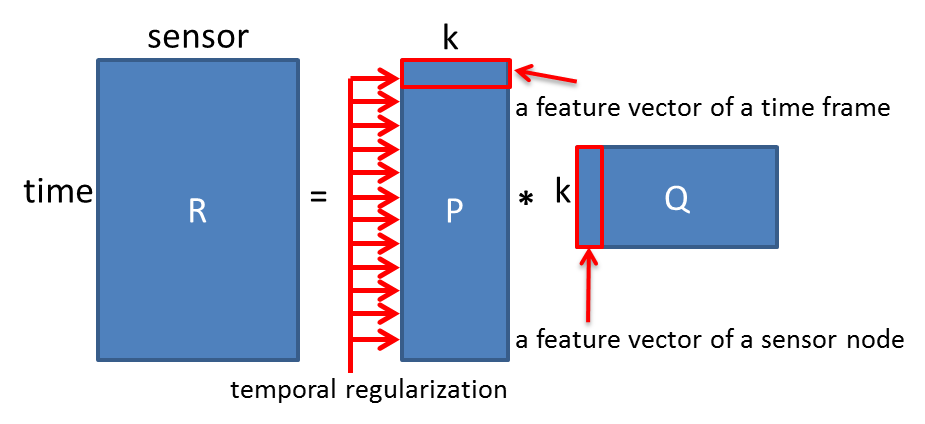
\includegraphics[width=0.4\textwidth]{TRMF_illustration.png}
	\caption{illustration of TR-MF}
\end{figure}
%cite temporal reference
Although we map the sensor data imputation task to a CF-based recommendation task, there are indeed some major differences in terms of the property of data.
Normal CF or MF models assume the users (i.e., temporal dimension) are independent of each other. That is, we can randomly swap the columns in the matrix without affected the factorization outcome. However, such independence does not exist in sensor data as a 
sensor's signal in time $t$ is highly dependent on that of time $t-1$. In other words, an ideal model should consider such order dependency, and under such a model the swap of columns shall significantly affect the outcome of factorization.

With this observation, we propose a Temporally-Regularized Matrix Factorization (TR-MF) to better model the characteristic of sensor data. As the name may suggest, TR-MF adds a temporal regularization term to conventional MF.
The temporal regularization forces the latent factors of adjacent rows to be similar, which reflects the fact that 
readings in adjacent time steps should be similar. We also add similar regularization term for row bias.
The modified objective function looks like: 
\begin{equation*}\small \begin{aligned}
\frac{1}{2}\sum_{m,n}{(r_{mn} - \hat{r}_{mn})}^2
&+ \frac{\beta}{2}(\sum_m{(\mu_m^2 + ||\mathbf{p}_m||^2)} + \sum_n{(\mu_n^2 + ||\mathbf{q}_n||^2)}) \\
&+ \frac{\gamma}{2} \sum{((\mu_m-\mu_{m+1})^2 + ||\mathbf{p}_m-\mathbf{p}_{m+1}||^2)}.
\end{aligned}\end{equation*}

\subsection{Spatio-Temporal-Regularized Matrix Factorization}
%A strong argument that directly exploiting spatial information to specify the assumed inter-sensor node correlation may not be as good as directly learning these correlations directly from the sensor observations themselves.
Although previously we argue that nearby sensors might not necessarily possess the highest correlation with each other, 
here we would like to show that our TR-MF model can easily be extended to accommodate spatial correlation if one decides to do so. 
Given the distance (or any kind of `closeness' measure) between sensors, we can add spatial regularization terms to bias for 
possible spatial correlation.
The objective function then becomes: 
\begin{equation*}\small \begin{aligned}
\frac{1}{2}\sum_{m,n}{(r_{mn} - \hat{r}_{mn})}^2
&+ \frac{\beta}{2}(\sum_m{(\mu_m^2 + ||\mathbf{p}_m||^2)} + \sum_n{(\mu_n^2 + ||\mathbf{q}_n||^2)}) \\
&+ \frac{\gamma_1}{2} \sum{((\mu_m-\mu_{m+1})^2 + ||\mathbf{p}_m-\mathbf{p}_{m+1}||^2)}\\
&+ \frac{\gamma_2}{2} \sum{((\mu_{n_i}-\mu_{n_j})^2 + ||\mathbf{p}_{n_i}-\mathbf{p}_{n_j}||^2)}.
\end{aligned}\end{equation*}
We call this Spatio-Temporal-Regularized Matrix Factorization (STR-MF). Note that we suggest users to exploit spatial 
regularization with care, as our experimental study will show that biasing for spacial correlation can often produce inferior results. 
In the following discussion, we will mainly focus on TR-MF.

\subsection{Optimization Procedure}
\label{optimation_procedure}
Several methods to learn MF have been proposed, such as Stochastic Gradient Descent (SGD)\cite{koren2009matrix,chih2008large}, Alternating Least Square (ALS)\cite{koren2009matrix,zhou2008large}, Newton's method\cite{buchanan2005damped} and Wiberg Algorithm\cite{okatani2007wiberg}.
For sensor data, we suggest SGD for its efficiency and simplicity. 

In SGD, we incrementally update our model by considering one reading at a time.
Focused on one observed reading $r_{mn}$ with the following objective function
\begin{equation*} \small \frac{1}{2}(r_{mn} - \hat{r}_{mn})^2
+ \frac{\beta}{2}(\mu_m^2 + \mu_n^2 + ||\mathbf{p}_m||^2 + ||\mathbf{q}_n||^2).\end{equation*}
It is not hard to derive the update equations as \\
\indent	$ \begin{cases} 
	\mu_m' = \mu_m - \eta ((\hat{r}_{mn}-r_{mn}) + \beta \mu_m) \\
	\mu_n' = \mu_n - \eta ((\hat{r}_{mn}-r_{mn}) + \beta \mu_n) \\
	\mathbf{p}_{m}' = \mathbf{p}_{m} - \eta ((\hat{r}_{mn}-r_{mn})\mathbf{q}_{n} + \beta \mathbf{p}_{m})\\
	\mathbf{q}_{n}' = \mathbf{q}_{n} - \eta ((\hat{r}_{mn}-r_{mn})\mathbf{p}_{m} + \beta \mathbf{q}_{n})\\
	\end{cases} $ \\
For each reading, we update all the $\mu_m$ and $\mathbf{p}_m$. Then after a full scan of all observed readings, 
we perform temporal regularization by updating all $\mu_m$ and $\mathbf{p}_m$ simultaneously according to the following equations:\\
\indent $ \begin{cases}
	\mu_m' = \mu_m - \eta \gamma_1((\mu_m-\mu_{m-1})+(\mu_m-\mu_{m+1}))\\
	\mathbf{p}_{m}' = \mathbf{p}_{m} - \eta \gamma_1((\mathbf{p}_{m}-\mathbf{p}_{m-1})+(\mathbf{p}_{m}-\mathbf{p}_{m+1}))\\
	\end{cases} $\\
The updating procedure is summarized in Procedure~\ref{alg:STRMF}. Note that we propose to avoid updating the temporal regularization with the update of each reading, because doing so can bias the model toward the time steps that possess fewer missing readings, which contradicts the goal of data imputation. 

If the spatial regularization is exploited, we can update all $\mu_n$ and $\mathbf{q_n}$ simultaneously as:\\
\indent $\begin{cases}
	\mu_{n_i}' = \mu_{n_i} - \eta \gamma_2 \sum_{n_j}{(\mu_{n_i} - \mu_{n_j})}\\
	\mathbf{q_{n_i}}' = \mathbf{q_{n_i}} - \eta \gamma_2 \sum_{n_j}{(\mathbf{q_{n_i}} - \mathbf{q_{n_j}})}\\
	\end{cases}$\\
where $n_i$ and $n_j$ is a pair of neighboring sensor nodes.

\paragraph*{Data Normalization}
Unlike the ratings in recommendation systems that are normally within certain range (e.g., 1 star to 5 star), readings from WSNs are real-valued (rounded to a desired level of precision), and the range may vary with the sensors.
Here we propose to normalize the training set to zero mean and unit variance before conducting MF learning, and once the missing values are produced by our model, we need to rescale the values to the original mean and variance.
Although this procedure does not change the quality of outcomes theoretically, in practice we do find some benefits: 
First, when the global mean becomes zero, the origin of our model naturally becomes a fine initial point for MF training, which is very important for non-convex optimization techniques such as MF.
Second, normalization forces different datasets to look similar, which simplifies the parameter tuning task. 


%\paragraph*{Parameters Setting}
%There are several parameters in our model: conventional regularization for user biases~$\beta_1$, item biases~$\beta_2$, user factors~$\beta_3$, item factors~$\beta_4$, temporal regularization for biases~$\gamma_1$ and for factors~$\gamma_2$, spatial regularization for biases~$\gamma_3$ and for factors$~\gamma_4$, learning rate for biases~$\eta_1$ and for factors~$\eta_2$, number of factors~$K$, and it can be time consuming to search for a good combination. 
%Here we provide some empirical suggestions to reduce the search space while still obtaining results with decent quality: the rule of thumb is to setup parameters of similar physical meanings to be identical. For example: the following setup is what we exploited for the experiments:
%$ \beta_1 = \beta_2 = \beta_3 = \beta_4, \gamma_1 = \gamma_2, \gamma_3 = \gamma_4, \eta_1 = \eta_2$. %\end{equation*}
%Advanced discussion on this aspect appears later in Section~\ref{subsec:parameter}.
%The parameters in our model are conventional regularization~$\beta$, temporal regularization~$\gamma$, learning rate~$\eta$, number of factors~$K$.
%A too small~$\eta$ or a too large~$K$ can slow down the training process, but it won't degrade the model.
\paragraph*{Stopping Criterion}
The validation set is used to determine the parameters and when to cease updating the MF model. More specifically, the training stops when the validation error keeps increasing for a certain amount of iterations (currently setup to $500$). 

\paragraph*{Time Complexity}
While training TR-MF, the time required for each update is $\Theta(KN + KR)$, where $K$ is the number of factors, $N$ is the number of observed readings and $R$ is the number of temporal and spatial regularization terms.
In other words, it is independent of the height and width of the data matrix. 
The total number of iterations varies with data quality, the missing rate and some parameters such as the learning rate and stopping criterion.
In our experiments, it normally takes several minutes to train a TR-MF model on a computer with Xeon 2.53GHZ processor and 16 to 64G memory, but in some circumstances the training time can grow to 1 to 2 hours.
To predict a missing value, it takes $2K$ multiplication operations, which can be done in real time. 
On a normal laptop, it takes less than one second to predict all values for our Berkeley data matrix ($270000$ values).
Note that we would like to emphasize that the training time is not as important as the prediction time, as normally we need only to train our model once to learn the optimal biases and factors for prediction.

\begin{algorithm}
	\caption{(Spatio-)Temporally-Regularized MF}
	\label{alg:STRMF}
	\textbf{Parameters:} $\beta$, $\gamma$, $\eta$, $K$\\
	\textbf{Input:} training set, validation set
	\begin{algorithmic}
		\State Normalize the training set as $\mathcal{D}$
		\State Initialize $\mu_m$, $\mu_n$, $\mathbf{p}_m$, $\mathbf{q}_n$ to small random numbers
		\Repeat
			\State \textbf{for} each observed reading $r_{mn}$ in $\mathcal{D}$
				\State \indent Update $\mu_m$, $\mu_n$, $\mathbf{p}_{m}$, $\mathbf{q}_{n}$
			\State Update $\mu_m$, $\mathbf{p}_m$ by temporal regularization
			\State (Update $\mu_n$, $\mathbf{q}_n$ by spatial regularization)
		\Until{stopping criterion is met}
		\State Output the model for testing set prediction
	\end{algorithmic}
\end{algorithm}

%\section{Tensor Factorization}  \label{sec:tf}

\section{Multivariate Factorization Model} \label{sec:tf}
A given sensor node may contain multiple sensor types and thus able to sense various aspects of its environment (e.g.\ temperature and humidity) at the same time.
These attributes may be correlated and this correlation may help in the missing data estimation process.
We propose two methods, Multivariate (S)TR-MF and Tensor Factorization, that leverage this multivariate correlation.

\subsection{Multivariate (S)TR-MF} %\label{subsec:Multivariate_TRMF}
If two matrices are correlated, then some of their latent factors should be similar.
This motivates us to design Multivariate (S)TR-MF.

Assume we have two attributes: temperature and humidity.
The $\mathbf{R}$ of Multivariate (S)TR-MF is the horizontal concatenation of the temperature matrix $\mathbf{R}_{tem}$ and $\mathbf{R}_{hum}$
\begin{equation*} \mathbf{R} = \begin{bmatrix}\mathbf{R}_{tem} & \mathbf{R}_{hum} \end{bmatrix} \end{equation*}

The objective function is similar to (S)TR-MF except that for each row (time step) there are two bias terms: one for temperature readings and the other for humidity readings.
Now $\mathbf{R}_{tem}$ and $\mathbf{R}_{hum}$ of $\mathbf{R}$ must be normalized independently with their own means and variances.
The optimization process remains the same as in Section \ref{optimation_procedure}.

Factorization models for tensors have been studied for many years~\cite{tg2009td}~\cite{bergqvist2010hosvd}. The main idea behind the use of Tensor Factorization (TF) is that we can take advantage of the principle behind Matrix Factorization to deal with additional features of the dataset. In sensor network data, temporal, spatial, and heterogeneous sensor information can be strongly correlated.
Modeling these correlation can thus be a great benefit when estimating missing values.
 
Tensor decomposition is a multi-dimensional extension of Singular Value Decomposition (SVD).
In the section \ref{sec:sensordecomp} we introduce the methods of Tensor Decomposition.
A general model of tensor decomposition is the Tucker decomposition (TD) also known as High-Order Singular Value Decomposition (HOSVD).
The special case of Tucker decomposition is called canonical decomposition (CD) also known as parallel factor analysis (PARAFAC).
Tensor Decomposition methods require a dense input matrix $\mathbf{R}$ with missing parts of input data ignored during optimization.
%Treating $\mathbf{R}$ as a dense tensor with missing entries being assume to be 0.
%It would make predict missing value failed.
We introduce and explain the details of how we have adapted the Tensor Decomposition models with latent factors for missing value estimation in Section \ref{sec:tfmissing}.
 
\subsection{Tensor Decomposition} \label{sec:tensordecomp}

 If we want to decompose a $m\times n$ Matrix M, recall the Singular Value Decomposition(SVD) as being
\begin{equation*} 
\mathbf{M}=\mathbf{P}\Sigma \mathbf{Q}^\mathrm{T}=\sum\limits_{k=1}^r\sigma_kp_kq_k^\mathrm{T}=\sum\limits_{k=1}^r\sigma_kp_k\otimes q_k
\end{equation*}
Where $\otimes$ denoted the tensor product : $x\otimes y = xy^\mathrm{T}$.
$r$ is the rank of $\mathbf{M}$,
$\mathbf{P}$ is an $m\times m$ unitary matrix, $\mathbf{Q}$ is a $n\times n$ unitary matrix, $\Sigma$ is an $m\times n$ rectangular diagonal matrix with singular values of M, being adopted the following convention $\sigma_1>\sigma_2 >...\sigma_r>0=\sigma_{r+1}=...=\sigma_{n}$.
The SVD may be generalized to High-Order Tensor decomposition.
the following are two types of tensor decomposition, for simplicity and in practical, we present the decomposition for 3-order tensor.

\subsubsection{Tucker Decomposition}
The Tucker decomposition was first introduced by Tucker in 1963 [1], it factorizes a higher-order tensor into a core tensor $\mathbf{S}$ and a factor matrix for each dimensions.
We decompose a $M\times N \times C $ tensor $\mathbf{T}$ :

\begin{equation*}
\mathbf{T}=\sum\limits_{i=1}^{I}\sum\limits_{j=1}^{J}\sum\limits_{k=1}^{K}\mathbf{S}_{ijk}p_i\otimes q_j\otimes w_k
\end{equation*}
or for each component,
\begin{equation*}
\mathbf{T}_{mnc}=\sum\limits_{i=1}^{I}\sum\limits_{j=1}^{J}\sum\limits_{k=1}^{K}\mathbf{S}_{ijk}\mathbf{P}_{m i}\mathbf{Q}_{n j}\mathbf{W}_{c k}
\end{equation*}
where the vectors $p_i$, $q_j$, and $w_k$ are the column of matrices $\mathbf{P}$, $\mathbf{Q}$ and $\mathbf{W}$ respectively, which are the factor matrices and usually orthogonal.
They can be thought of as the principal components in each order.
There are several algorithms for calculating Tucker decompositions.
For data compression, the Tucker decomposition usually assumes that $I\le M$, $J \le N $ and $K \le C$.

\subsubsection{Canonical Decomposition}

The Canonical decomposition factorizes a tensor into a sum of component rank-one tensors.
Formally, the Canonical Decomposition(CD) is the special case of the Tucker decomposition when $\mathbf{S}$ is superdiagonal.
The Canonical Decomposition of $\mathbf{T}$ is
\begin{equation*}
\mathbf{T}=\sum\limits_{k=1}^{K}x_k\otimes y_k\otimes z_k
\end{equation*}
or
\begin{equation*}
\mathbf{T}_{mnc}=\sum\limits_{k=1}^{K}\mathbf{X}_{m k} \mathbf{Y}_{n k} \mathbf{Z}_{c k}
\end{equation*}
where $x_i$,$y_i$ and $z_i$ are the column of matrices $\mathbf{X}$, $\mathbf{Y}$ and $\mathbf{Z}$, which are the factor matrices, $K$ is the factor size. 

The Tucker Decomposition and Canonical Decomposition are illustrated in Figure \ref{fig:tf:tuckcanon}.

\begin{figure}[h] 
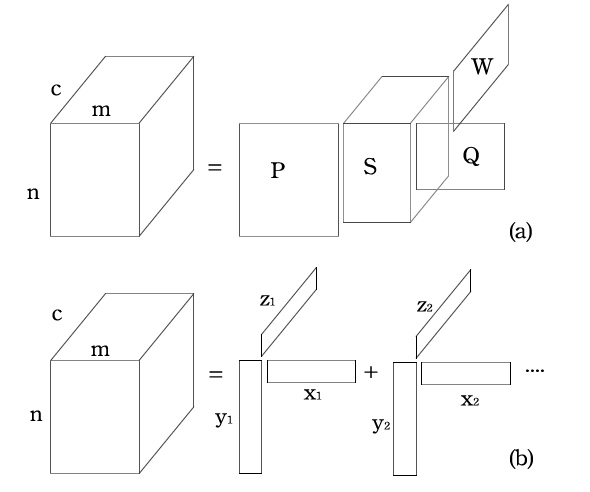
\includegraphics[width=9cm]{tf.jpg} 
\caption{ (a) the Tucker Decomposition (TD) model (b) the Canonical Decomposition model, a special case of the TD model.In sensor networks, the three dimension can be nominal features such as node id, time step index.} 
\label{fig:tf:tuckcanon} 
\end{figure}

\subsection{Tensor Factorization for Missing Data Estimation} \label{sec:tfmissing}
\subsubsection{Objective function}

Existing Tensor Decomposition models require a dense tensor, which is unsuitable for missing data estimation with a high missing rate. 
Therefore, we introduce an $N$-order Tensor Factorization for missing data estimation. In the CF technology, the TF also use in context-aware recommender system recently~\cite{karatzoglou2010multiverse}~\cite{steffen2010pairwise}~\cite{zeno2010context}.
Just like MF, it takes advantage of data sparsity while still exploiting the temporal correlation.
Moreover, it models the correlation between different information, e.g.\ spatial correlation and heterogeneous sensor readings.
The followings are the details of the model we propose.

Assume that there are three features $F_1, F_2 , F_3$, $F_1$ is the time step number, $F_2$ and $F_3$ are the other features, it could be the sensor node ID, sensor node coordinates, heterogeneous sensor readings or other information.
suppose the target sensor readings is $R$ such that tensor T containing  $R$ will be 3-dimensional tensor :
\begin{equation*}
\mathbf{T} := \mathbf{F_1} \times  \mathbf{F_2} \times \mathbf{F_3} \rightarrow \mathbf{R}
\end{equation*}

In contrast to conventional tensor decomposition, the learning model we propose is learning the latent factors $\mathbf{P}$,  $\mathbf{Q}$, $\mathbf{W}$.
Where $\mathbf{P}$,  $\mathbf{Q}$, $\mathbf{W}$ are the factors of $F_1, F_2, F_3$.
To avoid over-fitting and decrease the complexity of computing prediction, our model is based on Canonical Decomposition.
Its complexity of computing prediction is $\mathbf{O}(K)$, where K is the factor size of  P, Q and W.
On the other hand, the complexity of Tuker Decomposition is $\mathbf{O}(K^3)$  by our optimization method,
where $ K=min(K_P,K_Q,K_W) $ , $K_P$, $K_Q$, $ K_W$ are the factor size of $\mathbf{P}$,  $\mathbf{Q}$, $\mathbf{W}$ respectively.

As MF, to increase the prediction accuracy, we also add bias term of $F_1, F_2, F_3$ into our Tensor Factorization model.
so our prediction function is :
\begin{equation*}
\begin{aligned}
\mathbf{\hat{T}}_{mnc}=\mu_m+\mu_n+\mu_c+p_m \otimes q_n\otimes  w_c
\\=\mu_m+\mu_n+\mu_c+\sum\limits_{k=1}^{K}\mathbf{P}_{m k} \mathbf{Q}_{n k} \mathbf{W}_{c k}
\end{aligned}
\end{equation*}
to learn the latent features P, Q and W, we define the loss function :
\begin{equation*}
L(\mathbf{\hat{T}},\mathbf{T})=\frac{1}{\|\mathbf{D}\|_1} \sum\limits_{t\in \mathbf{D}}  l(\hat{t},t)
\end{equation*}
where $\mathbf{D}$ is the dataset and $\|\mathbf{D}\|$ means the amounts of data point.
$l$ is a point-wise loss function penalizing the distance between estimate and observation.
we choose $l$ being least squared error because the evaluation function is root mean square error (RMSE), so
\begin{equation*}
l(\hat{t},t)=\frac{1}{2}(t-\hat{t})^2
\end{equation*}

Simply minimizing a loss function is known to lead to over-fitting.
Given the factors P, Q, W and bias terms which constitute our model, we have a choice of ways to ensure that the model complexity does not grow without bound.
we add a regularization term based on the $l_2$ norm of these
factors.
To capture the temporal effect, similar to MF we state previous in section 3.2, we add the time regularization term to our model.
Finally, the objective function of tensor factorization is :\\
\begin{equation*}
\begin{aligned}
&\sum\limits_{m, n, c} l( \hat{\mathbf{T}}_{mnc}, \mathbf{T}_{mnc} )+\beta_1\|p_{\beta}\|^2+\beta_2\|q_n\|^2+\beta_3\|w_c\|^2+\beta_4\|
\mu_m\|^2\\
&+\beta_5\|\mu_n\|^2+\beta_6\|\mu_c\|^2+\frac{1}{2}\gamma_1\sum(\mu_m-\mu_{m+1})^2+(\mu_m-\mu_{m-1})^2
\\&
+\frac{1}{2}\gamma_2\sum(p_m-p_{m+1})^2+(p_m-p_{m-1})^2
\end{aligned}
\end{equation*}

\begin{algorithm}[h]
  \caption{Multivariate Tensor Factorization}
  \label{alg::conjugateGradient}
  \begin{algorithmic}[1]
    \Require
    $\beta_1,\beta_2, \beta_3, \beta_4, \beta_5, \beta_6, \gamma_1, \gamma_2, \eta, k$
    \State Normalize the training set as $D$
    \State initial the $p_m, q_n, w_c, \mu_m, \mu_n, \mu_c$ for all $m, n, c$
    \Repeat
      \For    {each observed readings t in D}
      \State Update $p_m, q_n, w_c, \mu_m, \mu_n, \mu_c$ 
     \EndFor
     \State Update $p_m,  \mu_m $ for all m
    \Until stopping criterion is met
    \State Output the model 
  \end{algorithmic}
\end{algorithm}

\subsubsection{Optimization}
Minimizing this objective function can be done using many approaches.
To deal with large datasets, there are simple and fast online algorithm which performs stochastic gradient descent (SGD) in the factors for a given tuple t simultaneously.
we need to compute the gradients of the objective function with respect individual components of the model.
Focus on a observed data t = $T_{m\beta\gamma } $ from training data, the update rule is :
\begin{equation*}
\begin{aligned}
&{p_m}^\prime={p_m}+\eta(e*q_n w_c - \beta_1 p_m)
\\&{q_n}^\prime={q_n}+\eta(e*p_m w_c - \beta_2 q_n)
\\&{w_c}^\prime={w_c}+\eta(e*p_m q_n - \beta_3 w_c)
\\&{\mu_m}^\prime=\mu_m+\eta(e-\beta_4\mu_m)
\\&{\mu_n}^\prime=\mu_n+\eta(e-\beta_5\mu_n)
\\&{\mu_c}^\prime=\mu_c+\eta(e-\beta_6\mu_c)
\end{aligned}
\end{equation*}
where $e=t-\hat{t}$, After a iteration, we update the model according to the temporal regularization :
\begin{equation*}
\begin{aligned}
&{p_m}^\prime={p_m}+\eta\gamma_1(p_{m+1}-p_m+p_{m-1}-p_m)
\\&{\mu_m}^\prime=\mu_m+\eta\gamma_2(\mu_{m+1}-\mu_m+\mu_{m-1}-\mu_m)
\end{aligned}
\end{equation*}
The Tensor Factorization method is summarized in Procedure 2, which is easy to implement since it accesses only one row of P, Q ,W at a time.

The details about normalization, initialization and stop criterion are just like MF, which are stated in previous part.
The parameters of TF are more than MF, but we can achieve reasonable performance by setting
\begin{equation*}
\begin{aligned}
& \beta_1=\beta_2=\beta_3=\beta_4=\beta_5=\beta_6\\
&\gamma_1=\gamma_2\\
\end{aligned}
\end{equation*}


\subsection{Multivariate Learning}
\subsubsection{Multivariate TRMF}

\begin{table}[htbp]
\caption{Multivariate RMSE (Berkeley, random)}
\label{traffic}
\begin{tabular}{r | r r r}
	&TRMF	&MtMF-Train	&MtMF-all \\ \hline
humid10-10-80	&0.1424	&0.1420	&0.1222\\
humid20-10-70	&0.1135	&0.1135	&0.0973\\
humid40-10-50	&0.0916	&0.0909	&0.0822\\
humid60-10-30	&0.0817	&0.0806	&0.0758\\
humid80-10-10	&0.0757	&0.0748	&0.0709\\
humid85-10- 5	&0.0751	&0.0739	&0.0712\\
 temp10-10-80	&0.1137	&0.1148	&0.0729\\
 temp20-10-70	&0.0462	&0.0481	&0.0369\\
 temp40-10-50	&0.0316	&0.0328	&0.0263\\
 temp60-10-30	&0.023	&0.0232	&0.0201\\
 temp80-10-10	&0.0182	&0.0183	&0.0166\\
 temp85-10- 5	&0.0153	&0.0154	&0.0143\\
\end{tabular}
\end{table}


\begin{table}[htbp]
\caption{Multivariate RMSE (Berkeley, temporal)}
\label{traffic}
\begin{tabular}{r | r r r}
	&TRMF	&MtMF-Train	&MtMF-all \\ \hline
humid10-10-80t	&0.957&0.996& 	0.991\\
humid20-10-70t	&0.796&0.852& 	0.846\\
humid40-10-50t	&0.771&0.835& 	0.807\\
humid60-10-30t	&0.540&0.887& 	0.880\\
humid80-10-10t	&0.447&0.483& 	0.480\\
humid85-10- 5t	&0.323&0.356& 	0.348\\
 temp10-10-80t	&0.515&0.567& 	0.555\\
 temp20-10-70t	&0.392&0.491& 	0.485\\
 temp40-10-50t	&0.310&0.380& 	0.347\\
 temp60-10-30t	&0.206&0.309& 	0.257\\
 temp80-10-10t	&0.132&0.429& 	0.432\\
 temp85-10- 5t	&0.088&0.122& 	0.114\\
\end{tabular}
\end{table}

\begin{table}[htbp]
\caption{Multivariate RMSE (traffic Data, Random)}
\label{traffic}
\begin{tabular}{r | r r r}
	&TRMF	&MtMF-Train	&MtMF-all \\ \hline
humid10-10-80	&3.524 	&3.486 	&2.291\\  
humid20-10-70	&2.583 	&2.558 	&1.796\\
humid40-10-50	&1.932 	&1.921 	&1.523\\
humid60-10-30	&1.664 	&1.649 	&1.408\\
humid80-10-10	&1.565 	&1.546 	&1.366\\
humid85-10- 5	&1.503 	&1.489 	&1.326\\
 temp10-10-80	&1.214 	&1.201 	&0.722\\
 temp20-10-70	&0.898 	&0.881 	&0.597\\
 temp40-10-50	&0.689 	&0.676 	&0.519\\
 temp60-10-30	&0.585 	&0.579 	&0.478\\
 temp80-10-10	&0.551 	&0.544 	&0.466\\
 temp85-10- 5	&0.520 	&0.510 	&0.434\\
\end{tabular}
\end{table}

\subsubsection{Tensor Factorization} % need to be combined with multi TRMF 
We compare our TF method with the models without modeling heterogeneous sensor correlations in this section.
The Tensor Factorization naturally allow us to add additional nominal dimensions to the model, e.g.\ node id or sensor coordinates.
The three-order TF is used in the experiment, each dimension represent node id, time frame number and heterogeneous signal.  
Due to the indexes of each dimension are discrete, the heterogeneous sensor data are not able directly used.
Therefore, the discretization of heterogeneous data is needed.
Before training, the heterogeneous signal are divide into some bins according to the value.
Each bin represents the index of the dimension.
Table ? and ? show the TF result of random split and temporal split on Berkeley dataset while table ? and ? show the TF result of random split and temporal split on traffic dataset.

\subsection{Prediction Performance}
In this section, we measure the performance of missing value recovery algorithms by regression methods.
We demonstrate the experiment on traffic dataset.
The readings of gateway node are to be predicted in offline mode.
At the sane time the data from gateway is the label of a instance while the data from the other sensor nodes are the features of a instance.
80 percent of instance are split to be training data, the remaining part is the testing data.
Firstly, we filling the features from training and testing data by global mean, linear interpolation, KNN, and TRMF model.
The regression model we choose is linear regression(LR) and support vector regression(SVR).
The former is a linear model.
In contrast, the latter is a nonlinear model.
Table ? show the result with different data missing rate.
It is obvious that the more higher quality filling value will help the regression model predicting the objective sensor more precise.

\begin{table} [htbp]
\centering
\caption{predict gateway humidity by LR (RMSE) }
\label{table: LR}
   Filling method
\begin{tabular}{ r | r r r r}
        missing rate&global mean     &LI   &Hybrid-KNN &TRMF\\ \hline
        5\%      &4.144&3.857&2.512&2.473\\
        10\%    &4.143&3.868& 2.597&2.526\\
        30\%    &5.161&3.955&2.773&2.470\\
        50\%    &6.234&4.282&3.158&2.756\\
        70\%   &7.728&5.082&3.310&2.743\\
        80\%   &9.019&7.458&3.306&2.802\\
\end{tabular}
\end{table}

\begin{table}[htbp]
\centering
\caption{predict gateway humidity by SVR (RMSE) }
\label{table: SVR}
   Filling method
\begin{tabular}{ r | r r r r}
        missing rate&global mean     &LI   &Hybrid-KNN &TRMF\\ \hline
        5\%&4.252&3.980&2.609&2.567\\
        10\%    &3.933 &4.006&2.749&2.591\\
        30\%    &5.172&4.083&2.814&2.532\\
        50\%    &6.234&4.384&3.260&2.813\\
        70\%   &7.686&5.235&3.313&2.822\\
        80\%  &9.039&8.508&3.464&2.910\\
\end{tabular}
\end{table}

\section{Discussion}  \label{sec:disc}

\subsection{Parameter Setting} \label{subsec:parameter}

We observe that the parameter setting for random split must be different from temporal split, and we provide an explanation for this. 

Let us look at two illustrating examples. Here we ignore bias terms for simplicity. Random split is like \textbf{Equation \ref{randomSplit_matrix}}. We have more confidence in our prediction and we rely more on temporal correlation, so we prefer more features and weak conventional regularization. Also, linear interpolation can be viewed as a solution of TRMF, in which the number of features is large and no conventional regularization is applied. 
\begin{equation}
\label{randomSplit_matrix}
\begin{bmatrix}
16 & 22 & 18\\
 ? & 22 & 19\\
18 &  ?	& 22\\
19 & 24 &  ?\\
20 & 26 & 26\\
\end{bmatrix} 
= 
\begin{bmatrix}
16 & 22 & 18\\
\mathbf{17} & 22 & 19\\
18 & \mathbf{23}	& 22\\
19 & 24 & \mathbf{24}\\
20 & 26 & 26\\
\end{bmatrix} 
\times
\begin{bmatrix}
1 & 0 & 0\\
0 & 1 & 0\\
0 & 0 & 1\\
\end{bmatrix} 
\end{equation}

Temporal split is like \textbf{Equation \ref{temporalSplit_matrix}}. We can't use temporal correlation to infer the missing values. We are less confident and we hope to apply the spatial correlation, so we prefer fewer features and stronger conventioal regularization.

\begin{equation}
\label{temporalSplit_matrix}
\begin{bmatrix}
30 & 30 & 28\\
31 & 31 & 28\\
32 &  ? & 28\\
33 &  ? & 28\\
32 &  ? & 28\\
\end{bmatrix} 
= 
\begin{bmatrix}
30 & 28\\
31 & 28\\
32 & 28\\
33 & 28\\
32 & 28\\
\end{bmatrix} 
\times
\begin{bmatrix}
1 & 1 & 0\\
0 & 0 & 1\\
\end{bmatrix} 
\end{equation}

To be specific, we share the actual values of the parameter. Firstly, the learning rate $\eta$ is $0.04$ to $0.004$, which is chosen as the largest value that still maintains stable optimization process. Secondly, a strong temporal regularization is always preferred. Temporal regularization times learning rate ($\gamma \times \eta$) is set to $0.2$ in all of our experiment. The conventional regularization is $0.001$ for temporal split and $0$ for random split. Finally, we observe that a large $K$ doesn't lead to overfitting because SGD is a natural regularization that prefers small feature values and it may lead to several non-independent features. The number of features $K$ is $54$ in Berkeley data set and $21$ in traffic data set, although in temporal split the $K$ may be much lowered to speed up the algorithm. 


\subsection{Parameter  WeiLun}
In temporal split data, it is more easier to be over-fitting state. Therefore, the regularization term should be higher than random split.
In experiment 4.3, it can be found TF works well on traffic dataset while it does't take advantage from adding heterogeneous signal on Berkeley dataset. Sensors from traffic dataset are deployed outdoor so the variance of heterogeneous data is large. While sensors from Berkeley dataset are deployed indoor, it cause the variance of heterogeneous data is small. The small variance makes TF does't work well because we quantize the heterogeneous signal into nominal bins before training. Most of heterogeneous sensor readings are divided into the same bin such that the additional dimension of TF is redundant.
We finally make a conclusion that the high variance heterogeneous data are suitable to use TF model but the low variance data are suitable to use Multiverse TRMF model. 

\subsection{Spatial Correlation}
One might wonder that why we don't apply spatial regulization to enhance the spatial correlation, like we did for temporal side.

\section{Conclusion}  \label{sec:conc}
This paper proposes the factorization-based models for missing data estimation. In contrast to many existing knowledge driven approaches which makes stronger assumptions about the data (e.g. assume that the closer sensor nodes have higher similarity; or assume the so-called neighborhood area is at the same radius away from the center in every direction), our factorization model is data driven that learns the inter-sensor and intra-sensor correlations through exploiting their latent similarity. Furthermore, we show that the additional knowledge such as the spatial relationships among sensor can seamlessly be incorporated into our model through regularization terms (e.g. STR-MF) if needed. Our experiments suggested that the temporal regularization is very helpful in general, while spatial information is useful only when the existing data are too little for the model to learn the inter-sensor relationships. Finally, we propose an update time $\Theta(KN + KR)$ multivariate tensor factorization model whose training complexity does not grow with its order, which allows the users to add arbitrary more dimensions or features into the imputation model without significantly increasing the computation burden.
We believe that the factorization models will become a very important kind of missing data recovery technique for WSN in the near future, and hopefully this paper can establish some foundation for more advanced research in this direction. 

\section{Acknowledgement} \label{sec:ack}

Acknowledgement here!



\balance
\bibliographystyle{abbrv}
\bibliography{sensys12}

\end{document}
